\section{\textcolor{Salmon}{Effektivität} \textcolor{red}{TODO: Titel}}
\label{ch:Diskussion:Effektivität}
...\\

\noindent
Grund für die Fehlerquote:\\
hier schon drauf eingehen, dass Fragestellungen ungünstig waren (s. \autoref{ch:Diskussion:Methodenkritik})\\
\textbf{Aufgabenstellungen waren nicht so relevant, deshalb schlechte Ergebnisse}
Relevanz der Fragen \autoref{fig:usability_test:genauigkeit-zeit_alt-neu} \autoref{fig:usability_test:genauigkeit-zeit_alle-richtige}\\

% **********************************************
------\\
% **********************************************
\textbf{Ausreißer machen das Ergebnis unschaf - mäh}
\textcolor{red}{TODO: weitere t-Tests von Aufgaben 2+3}\\
--> ?? hier? oder war das bei der Nutzerbefragung?

% *********************
%   Effektivität
% *********************
Aufgabenangemessenheit\\
----------------------\\
wenn bei 2 die beiden Ausreißer weggenommen werden, die andersrum bewertet haben, dann wird der Unterschied auch signifikant (s. \autoref{fig:hist_prümper_all})\\
Boxplot: \autoref{fig:pruemper_Aufgabenangemessenheit}\\

\noindent
Steuerbarkeit\\
-------------\\
wenn bei 3 alt die beiden Ausreißer weggenommen werden, die andersrum bewertet haben, dann wird der Unterschied auch signifikant (s. \autoref{fig:hist_prümper_all})\\
Boxplot: \autoref{fig:pruemper_Steuerbarkeit}\\

\noindent
Die Hypothesen die nicht bestätigt werden können\\
------------------------------------\\
gut für mich\\
--> können nicht bestätigte Hypothesen durch ungünstige Fälle doch bestätigt werden?\\
--> wird das Ergebnis noch signifikanter?\\
schlecht für mich\\
--> muss eine Gegendarstellung betrachtet werden?\\
--> wo führen Extrema zur Signifikanz, die sonst nicht da ist?\\

\noindent
Beispiele\\
---------\\
--> neuer t-Test weil Ausreißer, ist dann doch signifikant\\

\section{Woher kommen die Nutzerfehler?}
% ****************************************************************
%   Effizienz
% ****************************************************************
s.\autoref{fig:usability_effizienz}\\
--> bei Diskussion darauf eingehen, woher die höhere Fehlerquote kommt (in \autoref{fig:usability_test:genauigkeit-zeit_alt-neu})\\

\noindent
- Fehlergründe\\
Robustheit gegen Benutzungsfehler\\
% ISO_Benutzungsfehler
- in diesem Use-case nicht benötigt (es gibt keine Fehler-Anzeigen, s. \autoref{Add:Nutzerbefragung_Prümper:Begründung_Filterung})\\
- wird durch Usability-Test überprüft --> Fehlerquote\\
--> ABER: auf Fehlergründe eingehen\\
% weitere: Erwartungskonformität, Erlernbarkeit, Selbstbeschreibungsfähigkeit
- woher kommt die höhere Fehlerquote auf dem Dashboard\\
--> neue Anordnung (wurde vorher mal erwähnt) \autoref{ch:Dashboard:sec:Aufbau}??\\
\underline{Fehlerbetrachtung}\\
- Fehlende Daten aus Gründen xy\\

% Genauigkeit-Zeit
\begin{figure}[H]
    \centering
    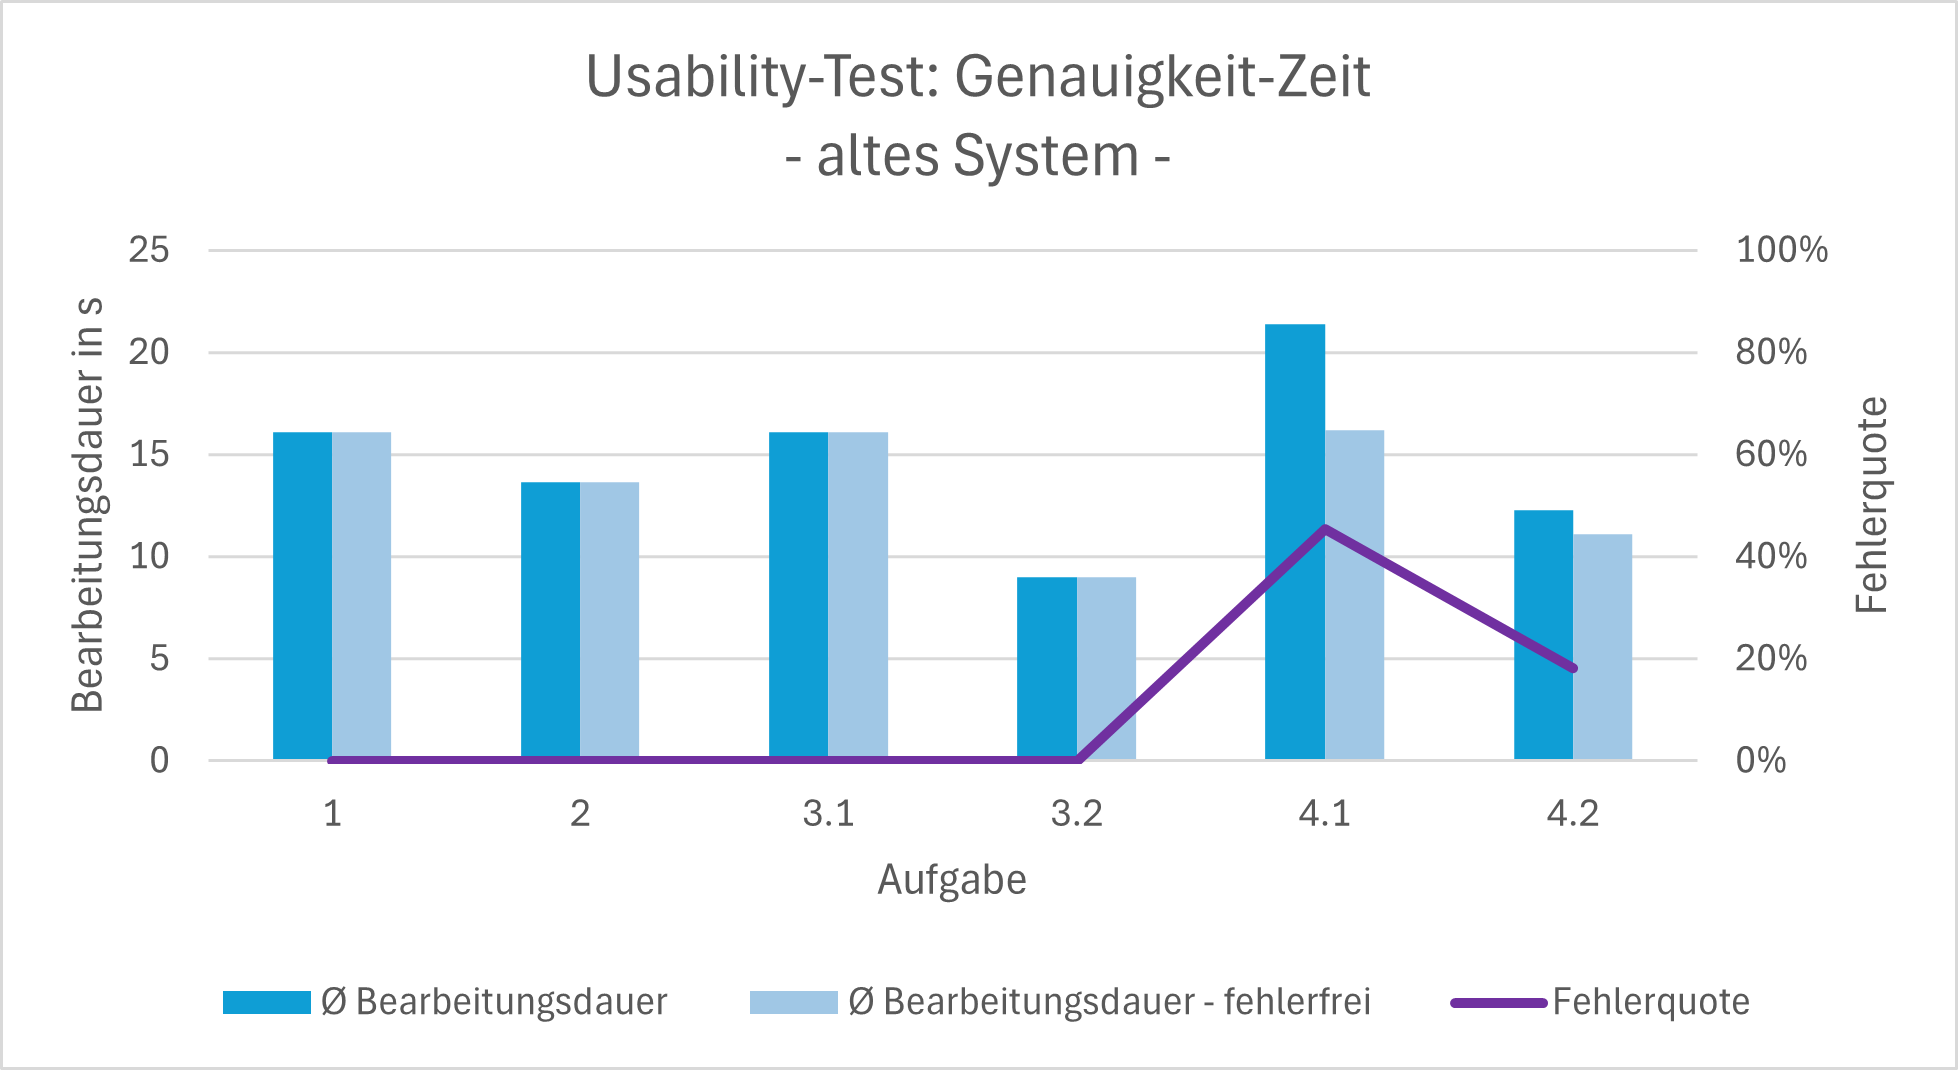
\includegraphics[width=0.8\linewidth]{Diagramme/usability_genauigkeit-zeit_alt.png}
    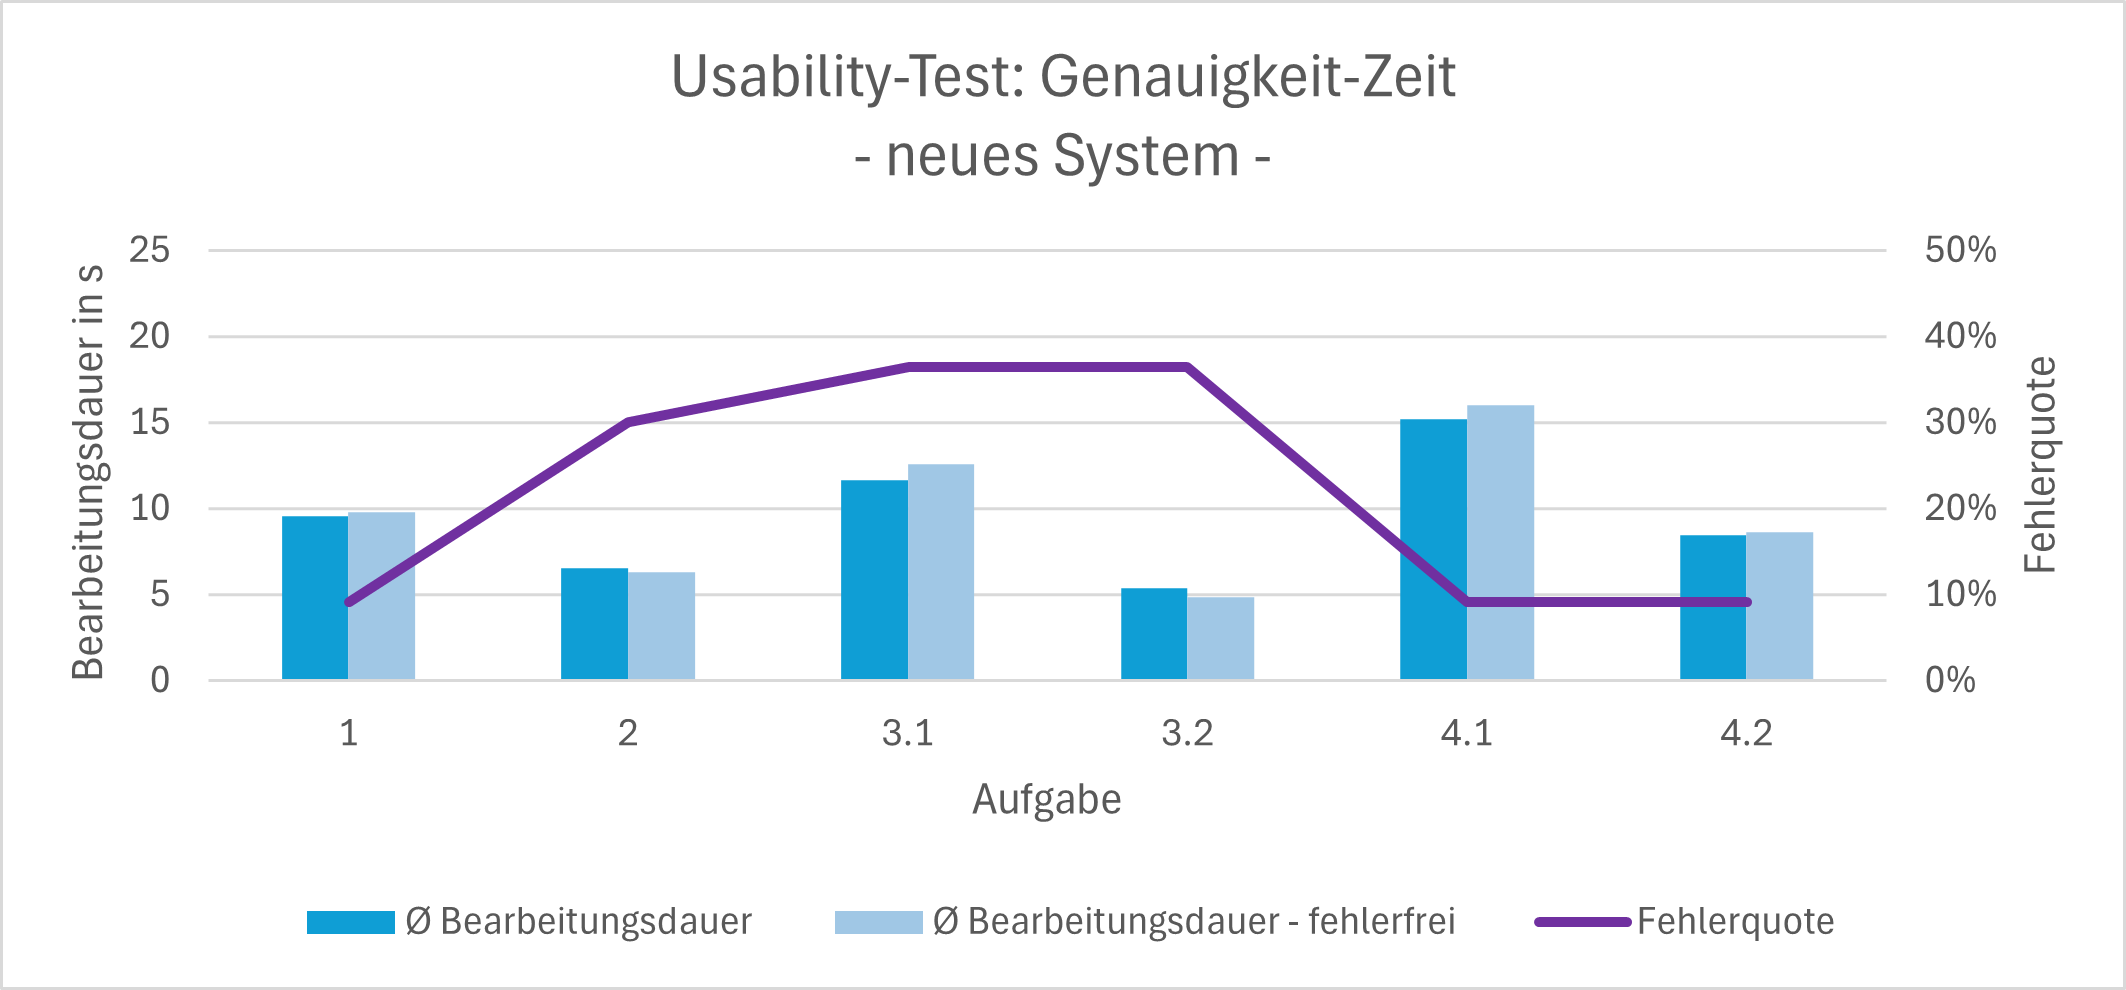
\includegraphics[width=0.8\linewidth]{Diagramme/usability_genauigkeit-zeit_neu.png}
    \caption{Usability-Test: Vergleich Genauigkeit-Zeit im alten und neuen System (Daten aus \autoref{tab:usability_test:mittelwerte})}
    \label{fig:usability_test:genauigkeit-zeit_alt-neu}
\end{figure}

\noindent
\underline{s. \autoref{fig:usability_test:genauigkeit-zeit_alt-neu}}\\
- alt: Leute mit Fehlern waren langsamer\\
- neu: Leute ohne Fehler waren minimal langsamer, kein signifikanter Unterschied\\
- neu: höhere Fehlerquote, dafür auch x\% schneller (Bsp. Frage 1: 15s auf 10s)\\
--> bei Diskussion darauf eingehen, woher die höhere Fehlerquote kommt

\begin{figure}[H]
    \centering
    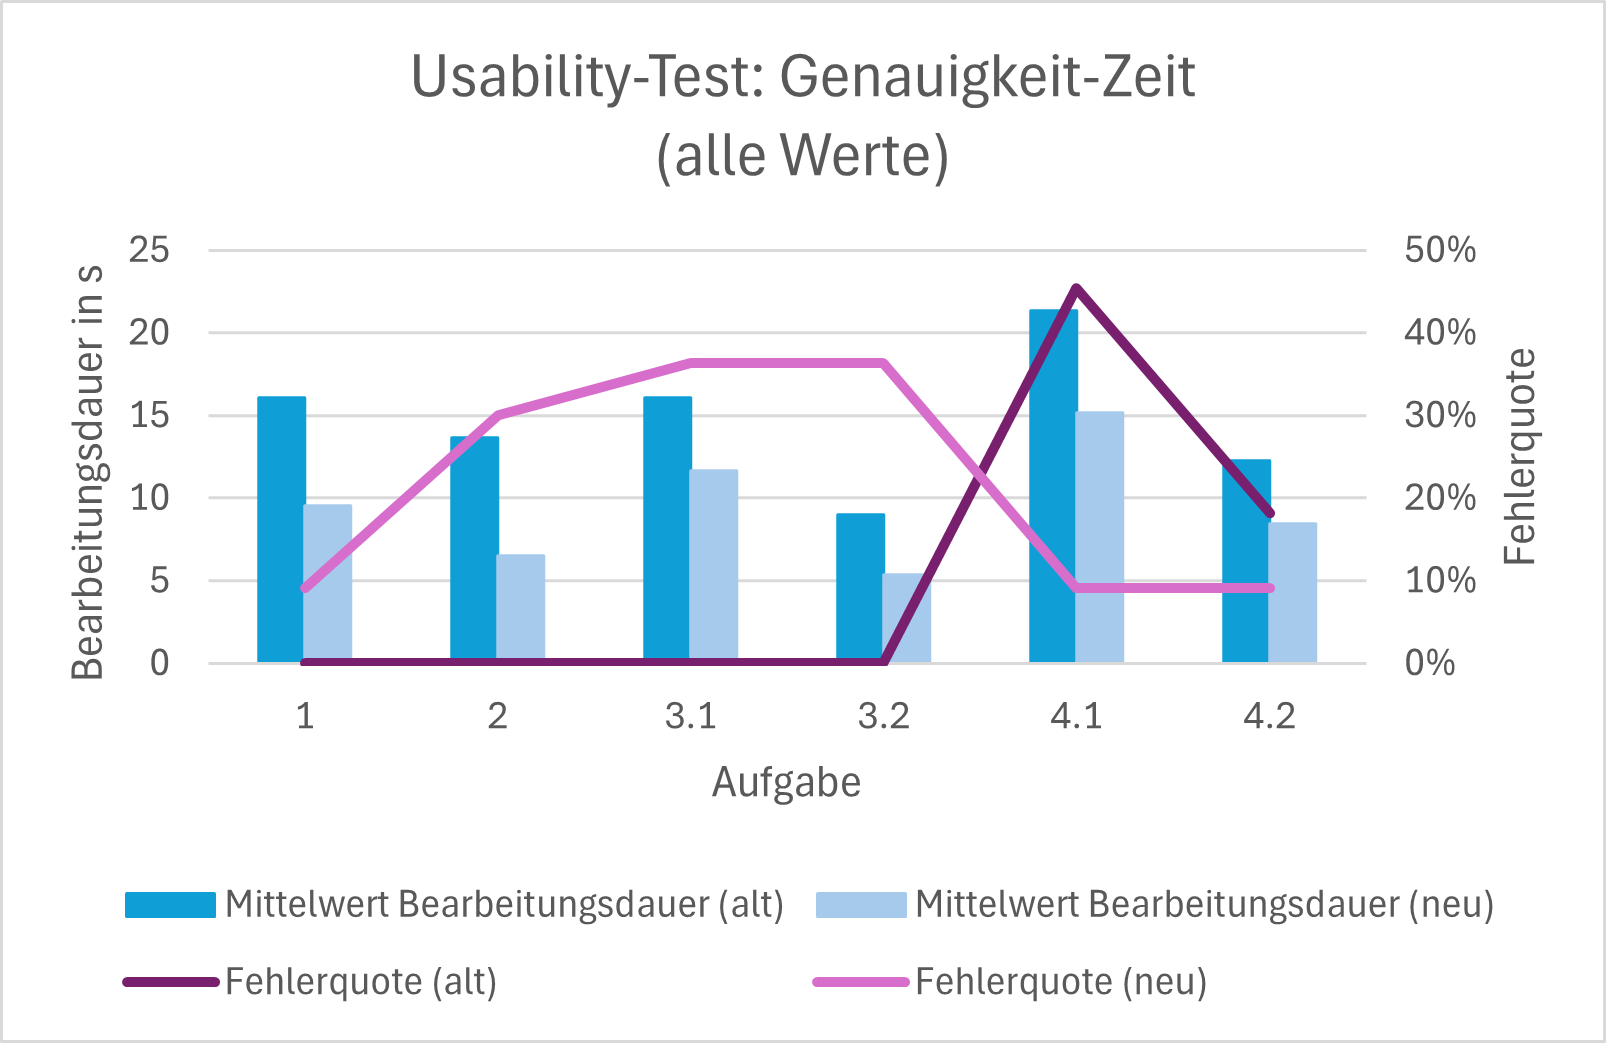
\includegraphics[width=0.8\linewidth]{Diagramme/usability_genauigkeit-zeit_alle.png}
    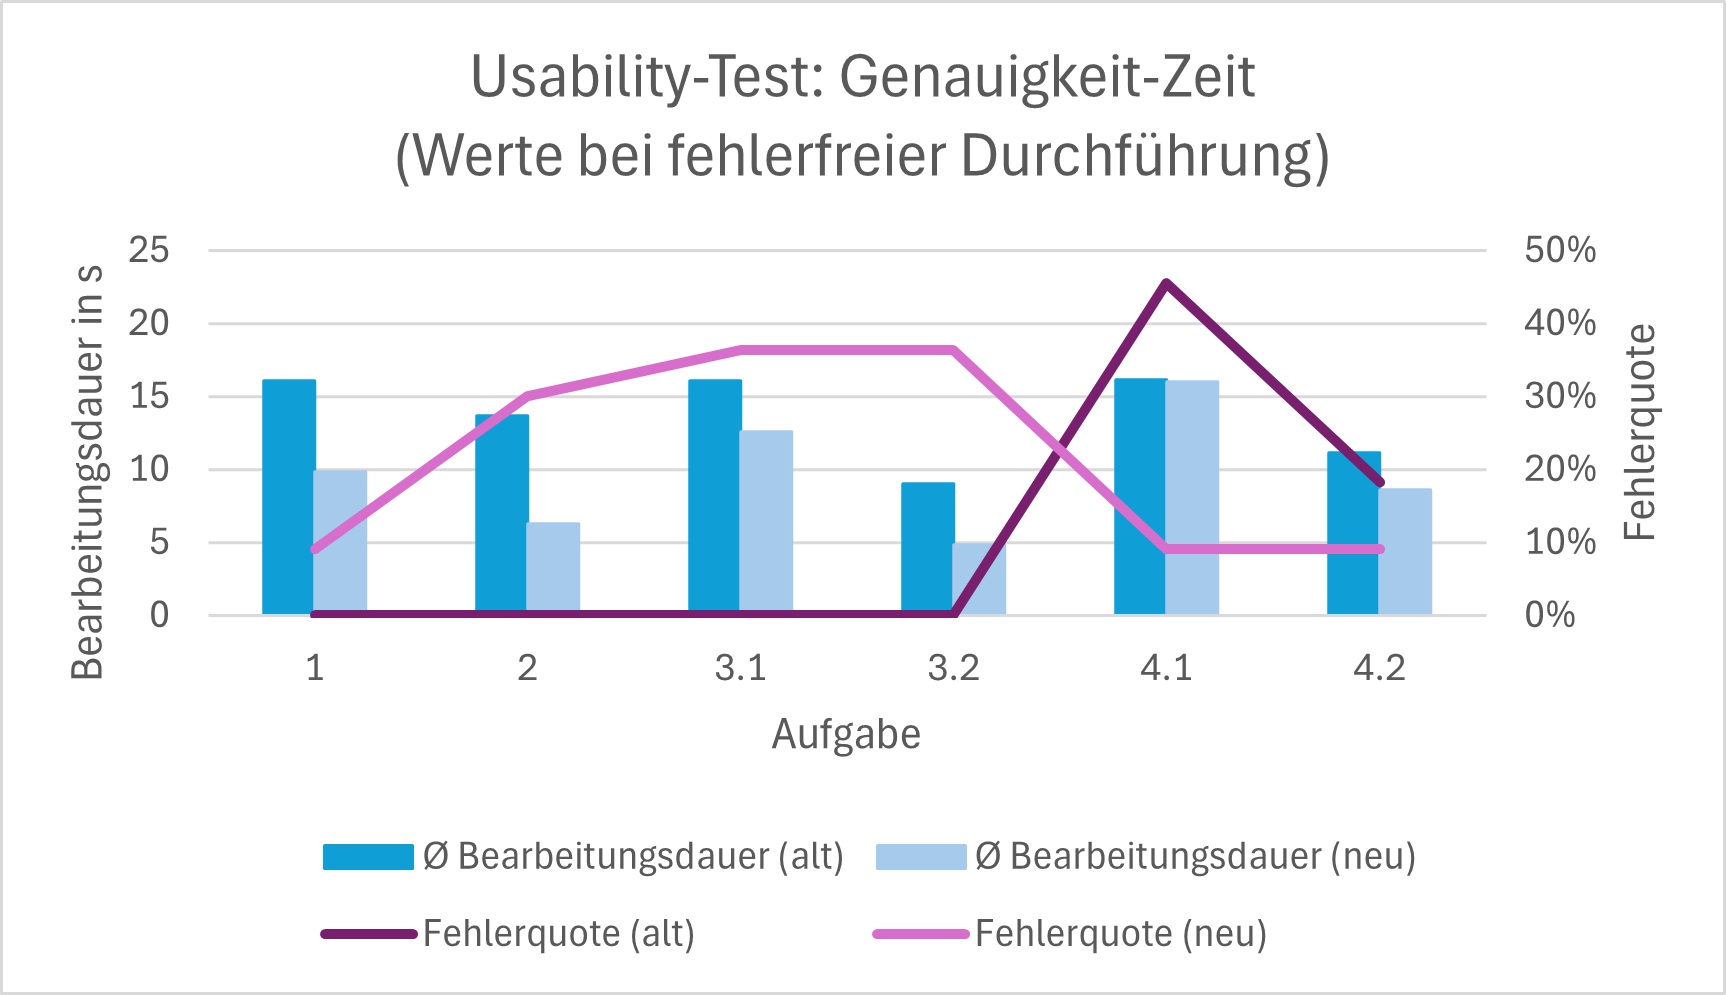
\includegraphics[width=0.8\linewidth]{Diagramme/usability_genauigkeit-zeit_richtige.png}
    \caption{Usability-Test: Zeitvergleich von allen Werten und nur richtigen Antworten - im Verhältnis zur Fehlerquote (Daten aus \autoref{tab:usability_test:mittelwerte})}
    \label{fig:usability_test:genauigkeit-zeit_alle-richtige}
\end{figure}

\noindent
\underline{s. \autoref{fig:usability_test:genauigkeit-zeit_alle-richtige}}\\
- neu ist in jeder Aufgabe ersichtlich schneller\\
--> Frage nach signifikanz\\
- Fehlerquote nicht überall eindeutig\\

\begin{itemize}
    \item Hypothese war … (beschreiben)\\
        --> kann hiermit bestätigt / wiederlegt werden
    \item es zeigt sich aber dass Person x mir ein Strich durch die Rechnung macht (Frage 2\&3 \autoref{fig:pruemper_ttest_frage_2} und \autoref{fig:pruemper_ttest_frage_3})
    \item die alten leute sind superschnell und total genau mit dem alten system (Effizienz)
    \item aber in der Zukunft lohnt es sich (evtl. Effizienz der jüngeren; alle außer die eingesessenen)
    \item ist sinnvoll die Mitarbeiter erstmal in ihrem Comfortbereich zu lassen, nicht direkt alles zu ändern (Zufriedenheit)
\end{itemize}

\noindent
- Fragen unverständlich formuliert\\
--> Leute mussten zu oft hin und her, könnte die Messdaten verfälscht haben\\
--> Methodenkritik?\\
